\begin{frame}[fragile]
\frametitle{Disassembly of $<$main$>$ (Part 1) with objdump}
\small
\begin{verbatim}
8049d05 <main>:
8049d05:       8d 4c 24 04             lea    0x4(%esp),%ecx
8049d09:       83 e4 f0                and    $0xfffffff0,%esp
8049d0c:       ff 71 fc                push   -0x4(%ecx)
8049d0f:       55                      push   %ebp
8049d10:       89 e5                   mov    %esp,%ebp
8049d12:       51                      push   %ecx
8049d13:       83 ec 34                sub    $0x34,%esp
8049d16:       89 4d e4                mov    %ecx,-0x1c(%ebp)
8049d19:       c7 04 24 cc a5 04 08    movl   $0x804a5cc,(%esp)
8049d20:       e8 37 ec ff ff          call   804895c <puts@plt>
8049d25:       e8 82 eb ff ff          call   80488ac <getuid@plt>
8049d2a:       85 c0                   test   %eax,%eax
8049d2c:       75 31                   jne    8049d5f <main+0x5a>
8049d2e:       a1 20 b4 04 08          mov    0x804b420,%eax
8049d33:       89 44 24 0c             mov    %eax,0xc(%esp)
8049d37:       c7 44 24 08 1a 00 00    movl   $0x1a,0x8(%esp)
8049d3e:       00
\end{verbatim}

\end{frame}

\begin{frame}[fragile]
\frametitle{Disassembly of $<$main$>$ (Part 2) with objdump}

\begin{verbatim}
8049d3f:       c7 44 24 04 01 00 00    movl   $0x1,0x4(%esp)
8049d46:       00
8049d47:       c7 04 24 42 a6 04 08    movl   $0x804a642,(%esp)
8049d4e:       e8 89 eb ff ff          call   80488dc <fwrite@plt>
8049d53:       c7 45 e8 01 00 00 00    movl   $0x1,-0x18(%ebp)
8049d5a:       e9 1c 03 00 00          jmp    804a07b <main+0x376>
8049d5f:       8b 55 e4                mov    -0x1c(%ebp),%edx
8049d62:       8b 42 04                mov    0x4(%edx),%eax
8049d65:       89 44 24 04             mov    %eax,0x4(%esp)
8049d69:       8b 55 e4                mov    -0x1c(%ebp),%edx
8049d6c:       8b 02                   mov    (%edx),%eax
8049d6e:       89 04 24                mov    %eax,(%esp)
8049d71:       e8 e2 f8 ff ff          call   8049658 <env_prepare>
8049d76:       e8 59 fa ff ff          call   80497d4 <y0y0stack>
8049d7b:       e8 b1 fa ff ff          call   8049831 <y0y0code>
\end{verbatim}

\end{frame}




\begin{frame}
\frametitle{Introduction Ghidra}

\begin{itemize}
    \item \textbf{Disassembly and Decompilation:}
    \begin{itemize}
        \item Transforms binary code into human-readable assembly.
        \item Generates high-level language representations (C-like pseudocode).
    \end{itemize}
    \item \textbf{Cross-Platform Support:}
    \begin{itemize}
        \item Analyzes binaries for multiple architectures (x86, ARM, MIPS, etc.).
        \item Compatible with various operating systems (Windows, Linux, macOS).
    \end{itemize}
    \item \textbf{Collaboration:}
    \begin{itemize}
        \item Supports multi-user reverse engineering projects.
        \item Version-controlled changes for shared analysis.
    \end{itemize}
    \item \textbf{Scriptability:}
    \begin{itemize}
        \item Customize and automate analysis with Python and Java.
    \end{itemize}
    \item \textbf{Extensibility:}
    \begin{itemize}
        \item Add plugins and extend functionality for specific needs.
    \end{itemize}
    \item \textbf{Data Flow Analysis:}
    \begin{itemize}
        \item Tracks variables, functions, and references for better insight.
    \end{itemize}
\end{itemize}

\end{frame}

\begin{frame}
\frametitle{Static Analysis Using Ghidra}
\begin{itemize}
    \item Creating a project in Ghidra.
    \item Importing and analyzing a binary file.
\end{itemize}

\centering
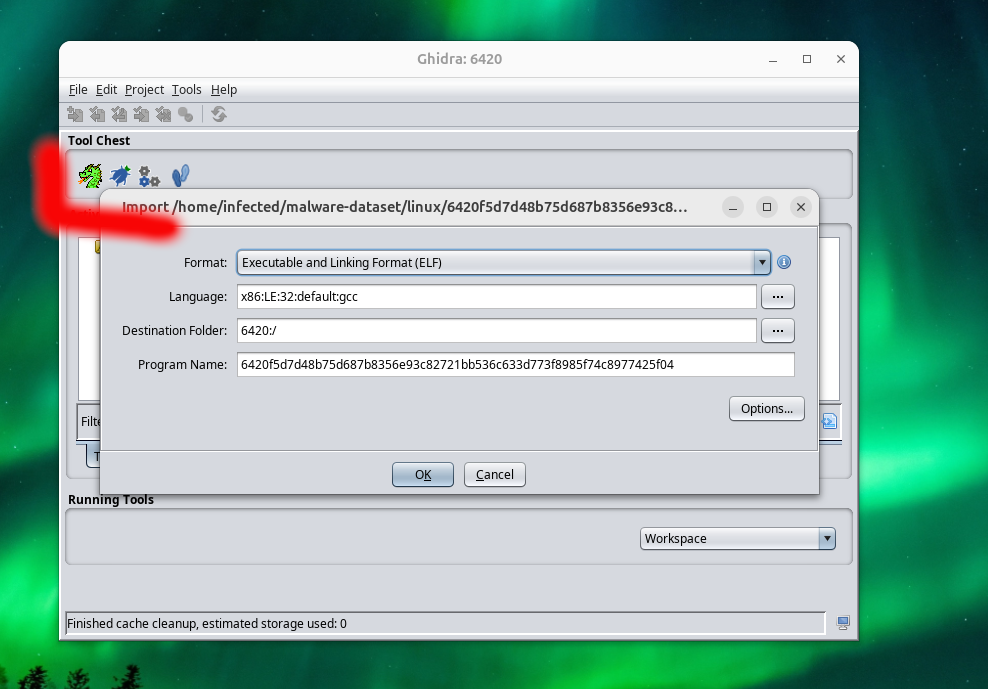
\includegraphics[width=0.6\textwidth]{img/g0.png}

\end{frame}

\begin{frame}
\frametitle{Static Analysis Using Ghidra}

\begin{itemize}
    \item Determine the type of binary (e.g., ELF, PE).
    \item Analyze the binary's metadata for key attributes such as architecture, endianness, and sections.
\end{itemize}

\centering
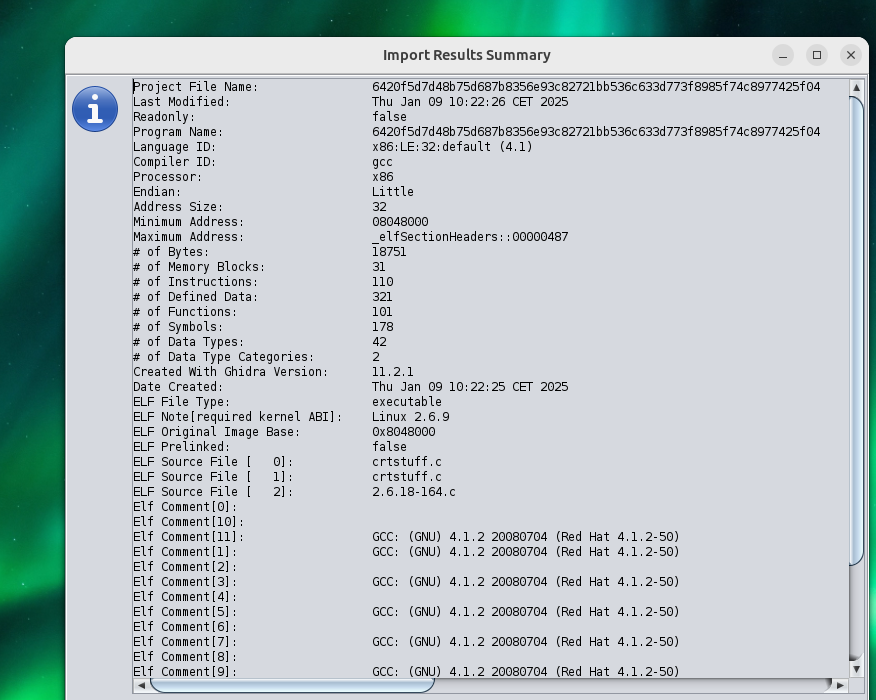
\includegraphics[width=0.6\textwidth]{img/g1.png}
\end{frame}

\begin{frame}
\frametitle{Static Analysis Using Ghidra}

\begin{itemize}
    \item Explore the functions defined within the binary.
    \item Analyze the disassembly view to examine low-level instructions.
    \item Utilize the decompiled view for a high-level representation of the code.
\end{itemize}

\centering
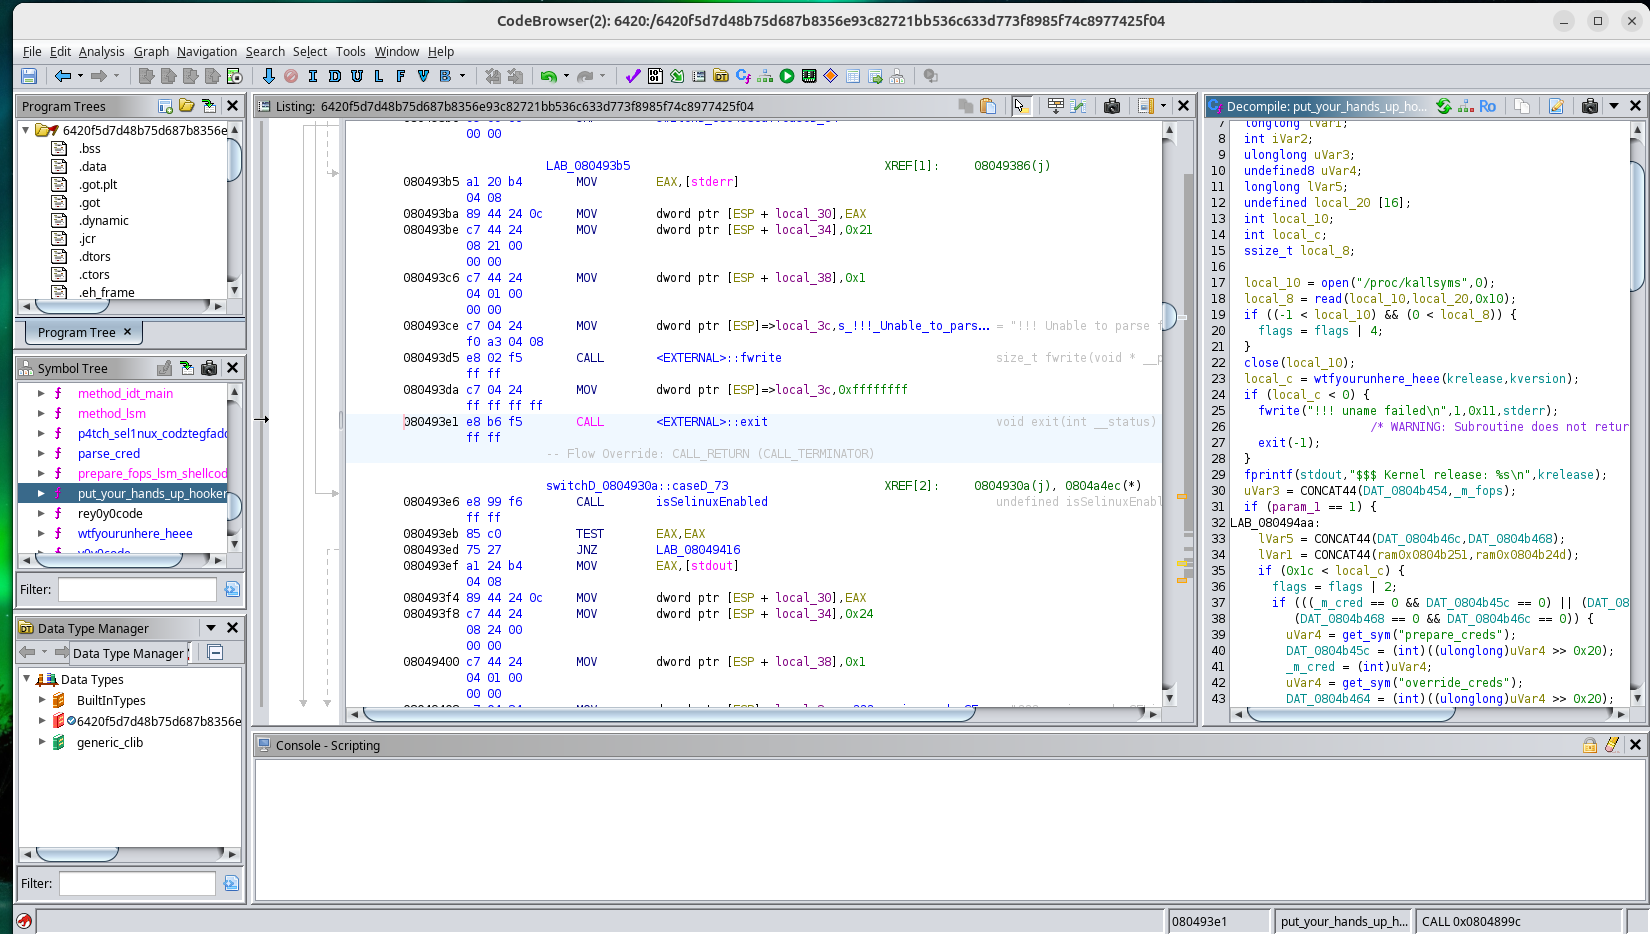
\includegraphics[width=0.6\textwidth]{img/g2.png}
\end{frame}

\begin{frame}
\frametitle{Static Analysis Using Ghidra}

\begin{itemize}
    \item \textbf{Benefits of Ghidra's Decompiled View:}
    \begin{itemize}
        \item Provides a high-level, human-readable representation of the code.
        \item Simplifies understanding of complex binaries.
    \end{itemize}
    \item \textbf{Avoid Manual Pattern Matching:}
    \begin{itemize}
        \item Eliminates the need to manually match patterns in assembly code.
        \item Speeds up the reverse engineering process.
    \end{itemize}
\end{itemize}

\centering
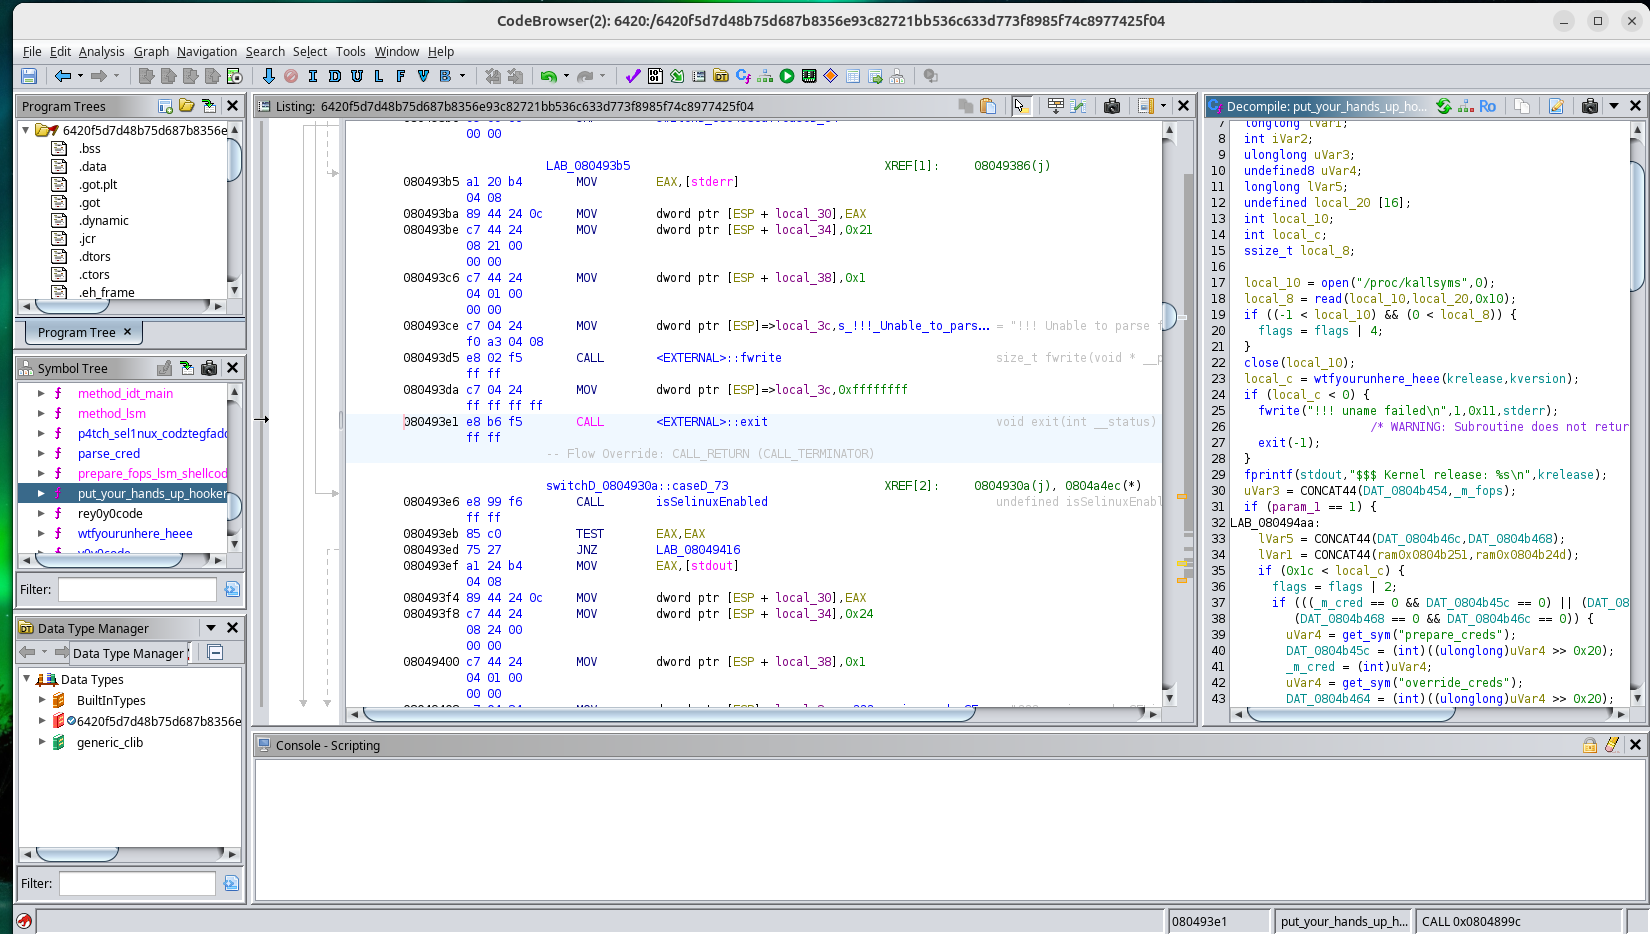
\includegraphics[width=0.6\textwidth]{img/g2.png}
\end{frame}

\begin{frame}
\frametitle{String Analysis and Cross-References in Ghidra}

\begin{itemize}
    \item Identify interesting strings, such as filenames, hardcoded paths, or error messages.
    \item Use the cross-references (Xrefs) feature to determine which functions or code sections utilize these strings.
\end{itemize}

\centering
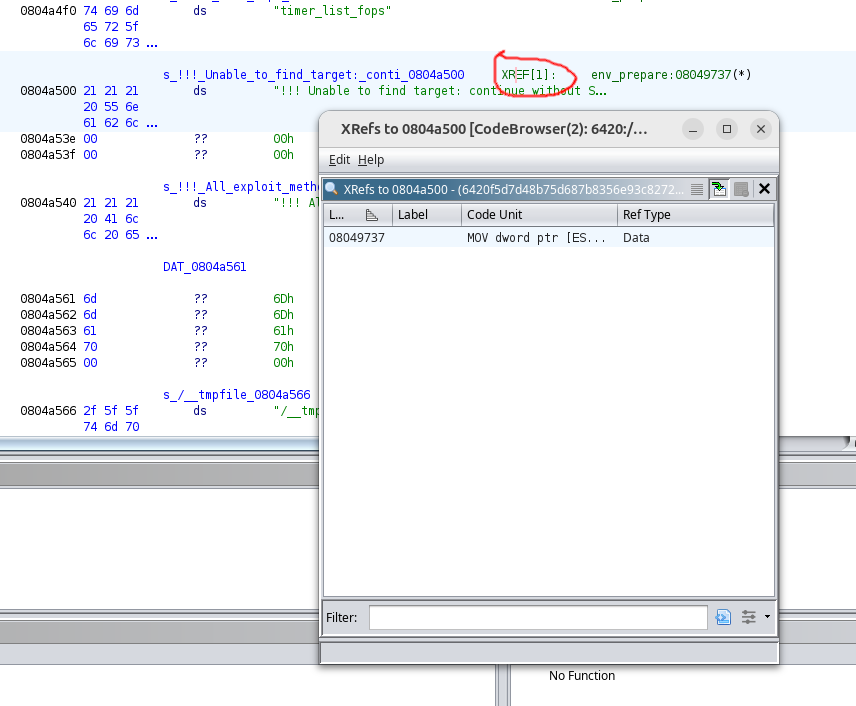
\includegraphics[width=0.6\textwidth]{img/gxref.png}
\end{frame}


\begin{frame}
\frametitle{String Analysis and Function Call Trees in Ghidra}

\begin{itemize}
    \item Certain functions are known to generate forensic artifacts, such as `fopen` and `mmap`.
    \item Locate these functions in the function call tree to identify which functions use them.
    \item Determine the artifacts that can be leveraged for detection and analysis.
\end{itemize}

\centering
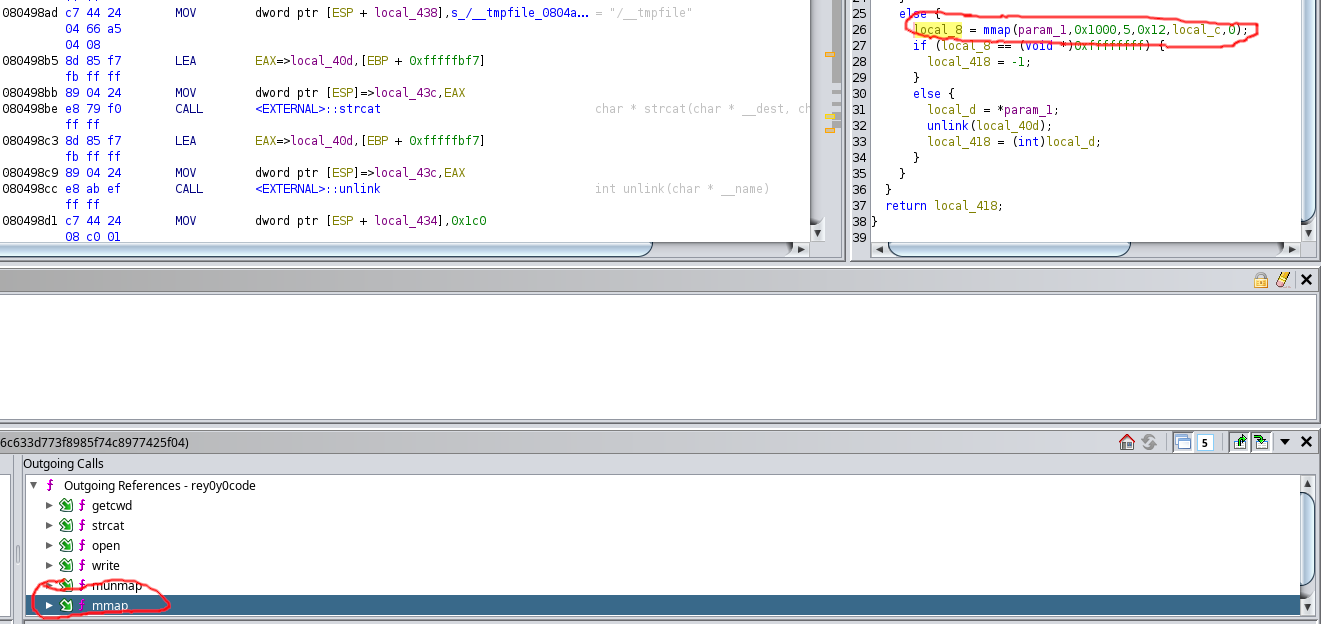
\includegraphics[width=0.6\textwidth]{img/goutcall.png}
\end{frame}


\begin{frame}
\frametitle{Static Analysis and Function Call Graphs in Ghidra}

\begin{itemize}
    \item Visual representations of function call graphs provide valuable insights into program behavior.
    \item Insights include identifying parsing activities, code execution loops, and function relationships.
\end{itemize}

\centering
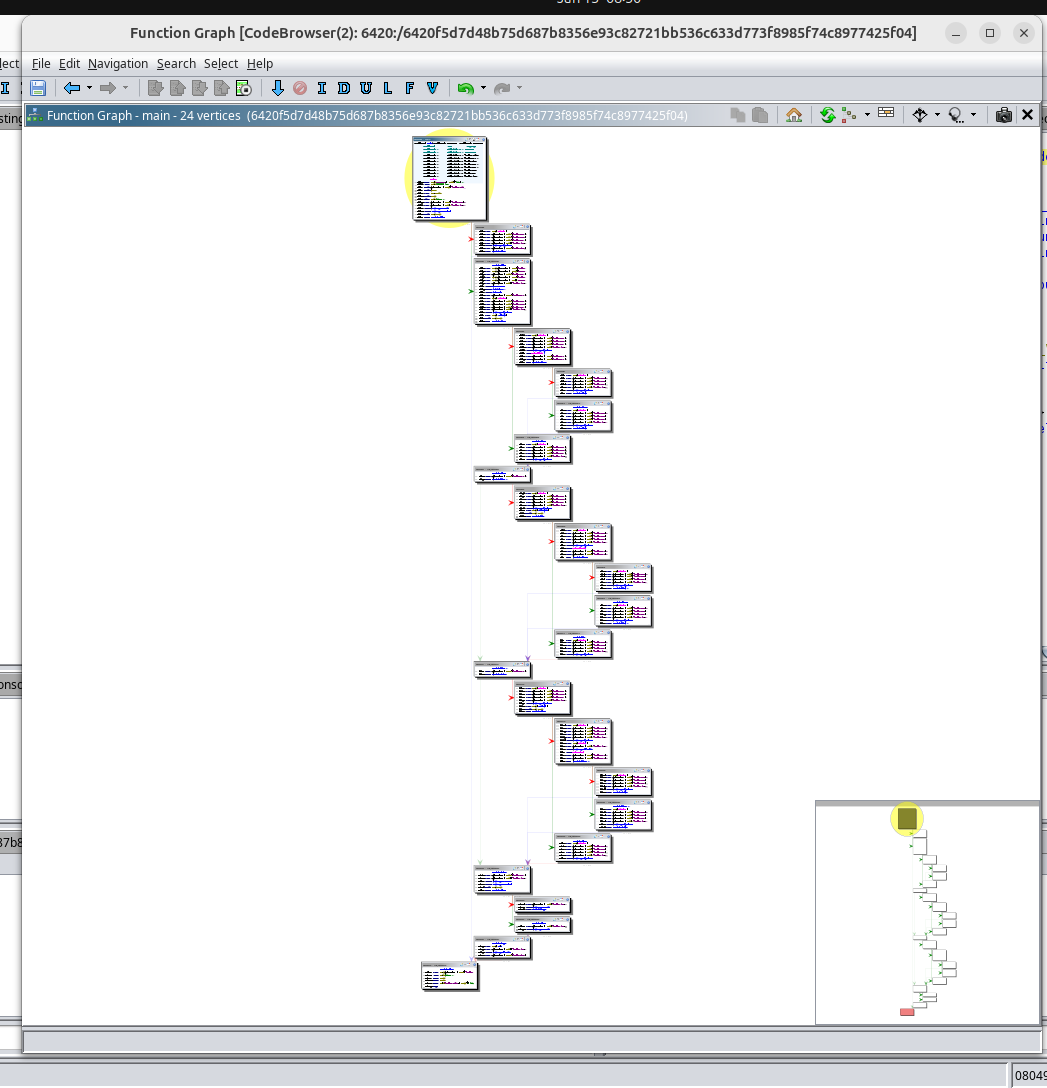
\includegraphics[width=0.6\textwidth]{img/gfctg.png}
\end{frame}
